\chapter{Web Semántica Geoespacial}
\label{ch:capitulo5}

\begin{quote}
	{\bf\textsc{Resumen:}} Este capítulo presenta la prueba de concepto realizada para la incorporación de Información Geográfica, procedente de Ogíjares (Granada), mediante herramientas de la Web Semántica. En el ejemplo se estudian y proponen herramientas de la Web Semántica que se pueden utilizar para representar e integrar datos geoespaciales con diferentes geometrías. Para realizar esta integración, se desarrolla la ontología GEOARES. 
\end{quote}



\section{Introducción a la prueba de concepto}

Como hemos comentado, uno de nuestros objetivos es estudiar las herramientas de la Web Semántica que se pueden utilizar para representar e incorporar Información Geográfica, valorarlas y desarrollar una prueba de concepto. Para ello se utilizarán los conceptos presentados en los capítulos dedicados a los sistemas SIG y a la Web Semántica, y así comprender que el principal nexo de unión entre ambas tecnologías es la estandarización de las operaciones y funciones usadas en las consultas de GeoSPARQL; tal y como hemos visto en el anterior capítulo. Conociendo todos estos conceptos es posible comenzar con el desarollo de la ontología GEOARES, sin embargo, la primera tarea imprescindible es la selección del conjunto de datos geoespaciales que se desea hacer accesible mediante la Web Semántica. \\

Durante la prueba de concepto contaremos y usaremos las herramientas destinadas a la generación de información geoespacial con \texttt{QGIS}, para permitir exportar la información de los \textit{Shapefile} a hojas de cálculo; generación de documentos \textit{RDF} con \texttt{Protegé}, para permitir llevar la información de los \textit{Shapefile} hacia documentos en formato \textit{RDF} de manera gráfica; consumo con \texttt{GraphBD},  para permitir la visualización de archivos en formato \textit{RDF} y la realización de las consultas con el lenguaje estándar de consulta geoespacial \textit{GeoSPARQL}; y visualización de la información geoespacial obtenida de las consultas con \texttt{R} para permitir ubicar la información geográfica en un mapa interactivo mediante la librería \textit{Shiny}.\\


% \texttt{QGIS} para permitir obtener la información de los \textit{Shapefile} a hojas de cálculo, generación de documentos \textit{RDF}  mediante \texttt{Protegé} para permitir llevar la información de los \textit{Shapefile} hacia documentos en formato \textit{RDF} de manera gráfica y su posterior visualización), consumo (mediante \texttt{GraphBD} para permitir la visualización de archivos en formato \textit{RDF} y la realización de las consultas del lenguaje estándar de consulta geoespacial \textit{GEOSPARQL}) y visualización de la información geoespacial obtenida de las consultas (\texttt{R} para permitir ubicar la información geográfica en un mapa interactivo mediante la librería \textit{Shiny}). 

\textit{\textbf{Nota}: La versión usada de QGIS es la 3.8.0-Zanzibar, la version de R es la 3.6.1, la versión de Protegé es la 5.5.0 y la versión de GraphDB Free es la 8.10.1, softwares usado en un macOS 10.14}

\section{Selección y obtención de los datos geográficos}
\label{ch:capitulo5-datos}

En la actualidad, disponemos de diversas fuentes oficiales y no oficiales que nos proporcionan mapas de calidad con los que poder trabajar. No obstante, al querer hacer uso de Información Geográfica de España, es importante destacar dos fuentes principales:

\begin{itemize}
	\item \textbf{Instituto Geográfico Nacional (IGN)}, es la fuente oficial para todo el territorio español y la descarga de mapas se puede realizar a través de la dirección \url{http://centrodedescargas.cnig.es/CentroDescargas/buscador.do#}.
	
	\item \textbf{Instituto de Estadística y Cartografía de Andalucía}, es la fuente oficial para todo el territorio andaluz y la descarga de mapas se puede realizar a través de la dirección \url{https://www.juntadeandalucia.es/institutodeestadisticaycartografia/bcadescargas/}.
\end{itemize}
 
Como vamos a trabajar con datos procedentes de la provincia de Granada, en concreto de mi pueblo, Ogíjares, he optado por escoger los que nos proporciona el \textit{Instituto de Estadística y Cartografía de Andalucía} \cite{base-andalucia}. A continuación, se muestran los pasos para su obtención:

\begin{enumerate}
	
		\begin{figure}[H]
		\centering
		\includegraphics[width=1\linewidth]{imagenes/capitulo5/obtencion-informacion}
		\caption{Portal del Instituto de Estadística y Cartografía \cite{base-andalucia}}
		\label{fig:obtencion-informacion}
	\end{figure}

	\item La descarga se realiza a través de la plataforma del Instituto de Estadística y Cartografía de Andalucía, de la Consejería de Economía y Conocimiento (URL mencionada en el punto anterior). Una vez dentro, seleccionamos la opción \texttt{Base Cartográfica de Andalucía (2)}, escogemos \texttt{Base Cartográfica de Andalucía (shape)} y buscamos el municipio de \textit{Ogíjares} (figura \ref{fig:obtencion-informacion}). Nos aparecerán varios cuadrantes, escogemos aquel con el que queramos trabajar; yo me he descargado el cuadrante que aparece seleccionado y remarcado en color, asociado a mi pueblo Ogíjares.
	
		\item La carpeta descargada contiene mapas de áreas muy diversas, las cuales hacen uso de geometría de punto, de línea o de polígono. Entre las capas que se nos proporcionan nos podemos encontrar diversos modelos de datos (tabla \ref{elementos-mapas}). \textit{Si queremos saber más debemos acceder a \url{https://www.juntadeandalucia.es/institutodeestadisticaycartografia/prodCartografia/bc/modelo.htm} y ``Nuevo modelo de datos''}.
			%\underline{\href{https://www.juntadeandalucia.es/institutodeestadisticaycartografia/prodCartografia/bc/modelo/00_Modelo_Datos_Base_Cartografica_Andalucia.pdf}{enlace}}.}
		



	
	
	
	\begin{table}[H]
		\caption{Esquema del modelo de datos descargado}
		\label{elementos-mapas}
		\centering
		\begin{tabular}{|m{6.2cm}|m{5.4cm}|}
			\hline
			\rowcolor[HTML]{EFEFEF} 
			\textbf{MODELO DE DATOS} & \textbf{ELEMENTOS} \\ \hline
			\textsc{Infraestructuras geográficas}&  Líneas administrativas            \\ \hline
			\textsc{Toponimia}&              Topónimos      \\ \hline
			\textsc{Relieve}&         Curvas de nivel, puntos de cota           \\ \hline
			\textsc{Sistema urbano}&       Edificaciones, curvas artificiales             \\ \hline
			\textsc{Servicios}&       Centros educativos o deportivos             \\ \hline
			\textsc{Red hidrográfica}&       Corriente artificial, punto fluvial  \\ \hline
			\textsc{Red viaria}&      Carreteras, carril bici              \\ \hline
			\textsc{Infraestructuras energéticas y de telecomunicaciones}&     Instalación de energía eléctrica, explotación minera               \\ \hline
			\textsc{Infraestructuras hidráulicas}&     Depósitos hidráulicos, presas               \\ \hline
			\textsc{Infraestructuras de transportes} &         Área de servicio de descanso       \\ \hline
			\textsc{Infraestructuras medioambientales} &     Instalación de tratamiento de aguas.               \\ \hline
			\textsc{Cubierta terrestre}&           Lindes        \\ \hline
		\end{tabular}
	\end{table}
	
				\begin{figure}[H]
		\centering
		\includegraphics[width=0.87\linewidth]{imagenes/capitulo2/shapefile}
		\caption{Diferentes archivos que componen el formato Shapefile }
		\label{fig:shapefile}
	\end{figure}

	\item El fichero descargado para cada uno de los modelos de datos que acabamos de comentar tiene como formato principal \textit{Shapefile (sh)}, el formato más usado para almacenar información geoespacial. Es un formato de archivos que almacena información no topológica con características espaciales de elementos geográficos que soporta geometrías como puntos, líneas y polígonos \cite{tesis}.  Es originario de \textit{Enviromental Systems Research Institute} (ESRI)\footnote{Empresa que desarolla y comercializa software para SIG.} y consta principalmente de un archivo principal, un archivo de índice y una tabla dBase; las demás extensiones son ficheros genéricos, como se puede ver en la figura \ref{fig:shapefile}. Estos archivos suelen requerir poco espacio de almacenamiento en disco y se pueden leer y escribir con facilidad. Los diferentes archivos que componen fundamentalmente el formato Shapefile tienen el mismo nombre cada uno con su respectiva extensión, como se aprecia en la figura \ref{fig:shapefile}:
	


	\begin{itemize}
		\item \textbf{Archivo principal (*.shp)}: archivo de longitud variable en el que cada registro describe una forma con sus respectivos vértices. 
		
		\item \textbf{Archivo de índice (*.shx)}: acompaña al archivo principal (*.shp) que almacena la posición de los identificadores de entidades individuales en el archivo .shp 
		
		\item \textbf{Tabla dBase (*.dbf)}: almacena la información de atributos de las entidades. 
	\end{itemize}	

	

	
	
	\item La visualización del archivo Shapefile se puede realizar a través de cualquier software SIG, en nuestro caso vamos a utilizar el software de análisis geoespacial QGIS. Respecto los modelos de datos disponibles que se desean escoger para hacer accesible mediante la Web Semántica, vamos a centrarnos en la información geoespacial de edificaciones, curvas de nivel y puntos de cota de Ogíjares (Granada) \cite{info-sh}, basados en el sistema de referencia ETRS89 (figura \ref{fig:codificacion}).
	

	

	\begin{figure}[H]
		\centering
		\includegraphics[width=0.56\linewidth]{imagenes/capitulo5/codificacion}
		\caption{Sistema de referencia usado en los Shapefiles}
		\label{fig:codificacion}
	\end{figure}

	\begin{itemize}
		\item \textbf{Edificaciones}: se agrupan en esta capa varios elementos que conforman edificaciones con geometría de polígono (figura \ref{fig:edificaciones}). Dispone de la información:
		
		\begin{itemize}
			\item \textsc{GID}.	
			\item \textsc{ID de la hoja}.
			\item \textsc{Estado}: estado de uso de la entidad o el tramo de la entidad.
			\begin{itemize}
				\item 	\small{En construcción (CON), en ruinas (RUI), sin clasificar (SCL) o en uso (USO).}
			\end{itemize}
			
			\item \textsc{Tipo}: tipo de elemento según su función.
			\begin{itemize}
				\item 	\small{Caseta o cobertizo (CAS), caso genérico (CGN), chabola (CHA), chimenea (CHI), edificación (EDI), industrial (IND), invernadero (INV), marquesina (MAR), nave abierta (NAB), nicho (NIC), patio (PAT), sin clasificar (SCL), tentadero (TEN), torre genérica (TGN), transformador (TRF) o torre de vigía (TVG).}
			\end{itemize}
			 
		\end{itemize}
	
		\begin{figure}[H]
		\centering
		\includegraphics[width=1\linewidth]{imagenes/capitulo5/edificaciones}
		\caption{Visualización del elemento \textit{Edificaciones} en QGIS}
		\label{fig:edificaciones}
	\end{figure}

		
		
		\item \textbf{Curvas de nivel}: línea imaginaria de altitud constante que sirve para describir la forma tridimensional de la superficie terrestre con geometría de línea (figura \ref{fig:curvasnivel}). Dispone de la información:
		
		\begin{itemize}
			\item \textsc{GID}.	
			\item \textsc{ID de la hoja}.
			\item \textsc{Cota}: recoge la coordenada altura ortométrica del elemento capturado en metros.
			\item \textsc{Categoría}: categoría de la curva de nivel.
			\begin{itemize}
				\item 	\small{Auxiliar (AUX), maestra (MAE), normal (NOR) o sin clasificar (SCL).}
			\end{itemize}
			
			\item \textsc{Procedencia}: procedencia de la curva de nivel.
			\begin{itemize}
				\item 	\small{Combinado (CMB), elementos terreno (ETE), lidar (LID), MDT (MDT), restitución (RES) o sin clasificar (SCL).}
			\end{itemize} 
			\item \textsc{Tipo}: tipo de la curva de nivel.
			\begin{itemize}
				\item 	\small{Caso genérico (CGN), depresión (DEP) o sin clasificar (SCL).}
			\end{itemize}
			
		\end{itemize}
	
	\begin{figure}[H]
		\centering
		\includegraphics[width=1\linewidth]{imagenes/capitulo5/curvasnivel}
		\caption{Visualización del elemento \textit{Curvas de Nivel} en QGIS}
		\label{fig:curvasnivel}
	\end{figure}
		
		
		
		
		\item \textbf{Punto cota}: punto situado sobre la superficie terrestre del cual se conoce su altitud sobre el nivel medio del mar, y que se representa para facilitar la interpretación gráfica de la morfología del terreno con geometría de punto (figura \ref{fig:puntocota}). Dispone de la información:
		
		\begin{itemize}
			\item \textsc{GID}.	
			\item \textsc{ID de la hoja}.
			\item \textsc{Cota}: recoge la coordenada altura ortométrica del elemento capturado en metros.
			\item \textsc{Contexto}: contexto del punto de cota.
			\begin{itemize}
				\item 	\small{Caso genérico (CGN), cima (CIM), collado (COL), depresión (DEP), edificación (EDI) o sin clasificar (SCL).}
			\end{itemize}
	

		\item \textsc{Tipo}: tipo de elemento según su función.
		
		\begin{itemize}
			\small{
			\item Punto cota construcción elevada (CON) o punto cota terreno (TER).
		}\end{itemize}
	\end{itemize}
	\end{itemize}

	\begin{figure}[H]
		\centering
		\includegraphics[width=0.95\linewidth]{imagenes/capitulo5/puntocota}
		\caption{Visualización del elemento \textit{Punto Cota} en QGIS}
		\label{fig:puntocota}
	\end{figure}
\end{enumerate}

\begin{figure}[H]
	\centering
	\includegraphics[width=1\linewidth]{imagenes/capitulo5/mapa}
	\caption{Visualización de las tres geometrías en QGIS}
	\label{fig:mapa}
\end{figure}

\textit{\textbf{Nota}: Estos ficheros se encuentran en el directorio \texttt{datos<shapefile}.}

Con esto se han presentado los datos que vamos hacer accesibles a través de la Web Semántica. En la figura \ref{fig:mapa} es posible visualizar las tres geometrías juntas y localizadas en QGIS a través de la capa \textit{OpenStreetMap}, en donde las líneas verdes hacen referencia a las curvas de nivel, los puntos rojos a los puntos de cota y los polígonos azules a las edificaciones. Por tanto, al disponer de los datos listos para su uso, es necesario saber que para poblar una ontología con Protegé, se necesitan los datos geoespaciales en formato para CSV. Adicionalmente, como hemos visto, la representación de la ubicación de cada geometría la vamos a usar mediante la codificación WKT. No obstante, QGIS nos ofrece diversas funcionalidades, entre las que se encuentran las anteriores mencionadas y que nos permiten realizar el trabajo de una manera más sencilla.\\ 

%Se han propuesto otros esquemas para codificar datos de geometría simple en RDF. El vocabulario de Geografía básica del W3C (http://www.w3.org/2003/01/geo/) es un vocabulario popular. Estos vocabularios simples tienen limitaciones, por ejemplo, la incapacidad de especificar diferentes datos y sistemas de coordenadas, y por lo tanto no se usaron en GeoSPARQL. Tenga en cuenta que la mayoría de los datos de geometría existentes codificados con estos vocabularios se pueden convertir fácilmente en representaciones GeoSPARQL. La consulta SPARQL a continuación crea valores geo: wktLiteral a partir de geometrías de geografía básica del W3C.


%Esta sección establece los requisitos para representar datos de geometría en RDF basados en WKT según lo definido por Características simples [ISO 19125-1].

%Todos los literales RDFS de tipo geo: wktLiteral consistirán en un URI opcional que identifica el sistema de referencia de coordenadas seguido de Texto bien conocido de características simples (WKT) que describe un valor geométrico. Geo válido: wktLiterals se forman concatenando un URI absoluto válido como se define en [RFC 2396], uno o más espacios (carácter Unicode U + 0020) como separador y una cadena WKT como se define en Características simples [ISO 19125-1 ]

Para obtener el formato CSV en QGIS se realiza el mismo proceso en las tres capas: \textit{click derecho sobre la capa en cuestión}, \texttt{Exportar>Guardar objetos como} y nos aparecerá una ventana como la de la figura \ref{fig:csv}. Además, para obtener la codificación WKT y poder hacer consultas a partir de la ubicación de las geometrías, debemos seleccionar en GEOMETRY la opción AS\_WKT (figura \ref{fig:opciones}) y ya podemos guardar los CSV (figura \ref{fig:guardar}). En las tablas \ref{csv-curva1}, \ref{csv-curvas2},\ref{csv-puntos} y \ref{csv-poligonos} se muestran fragmentos de dichos CSV.



\begin{table}[H]
	\centering
	\caption{Parte del CSV para Curvas de Nivel I}
	\label{csv-curva1}
	\begin{tabular}{|m{4.2cm}|c|c|c|c|}
		\hline
		\rowcolor[HTML]{EFEFEF} 
		\textbf{WKT} & \textbf{GID} & \textbf{ID} & \textbf{TIPO} & \textbf{CATEGORIA}  \\ \hline
		LINESTRING (440675.4 4106319.93, ....)       & 122602       & 102632            & CGN           & NOR                           \\ \hline
		LINESTRING (440972.5 4106237.28, ...)     & 172684       & 102632            & CGN           & NOR                       \\ \hline
		LINESTRING (440976.2 4106311.24, ...)              & 186391       & 102632            & CGN           & NOR                        \\ \hline
		...                                & ...       & ...            & ...           & ...                      \\ \hline
		
		LINESTRING (442507.6 4105386.75, ...)             & 471150       & 102632            & DEP           & MAE                       \\ \hline
	\end{tabular}
\end{table}

\begin{table}[H]
	\centering
	\caption{Parte del CSV para Curvas de Nivel II}
	\label{csv-curvas2}
	\begin{tabular}{|m{4.2cm}|c|c|c|}
		\hline
		\rowcolor[HTML]{EFEFEF} 
		\textbf{WKT}  & \textbf{PROCEDENCIA} & \textbf{COTA} \\ \hline
		LINESTRING (....)                  & CMB                 & 770           \\ \hline
		LINESTRING (...)                   & CMB                 & 780           \\ \hline
		LINESTRING (...)                      & CMB                 & 780           \\ \hline
		...                                & ...       & ...                  \\ \hline
		
		LINESTRING (...)                              & CMB                 & 750           \\ \hline
	\end{tabular}
\end{table}

\begin{table}[H]
	\centering
	\caption{Parte del CSV para Puntos de Cota}
	\label{csv-puntos}
	\begin{tabular}{|m{3cm}|c|c|c|c|c|}
		\hline
		\rowcolor[HTML]{EFEFEF} 
		\textbf{WKT}                        & \textbf{GID} & \textbf{ID} & \textbf{TIPO} & \textbf{CONTEXTO} & \textbf{COTA} \\ \hline
		MULTIPOINT ((446228.92 4108432.53)) & 890947       & 102632            & TER           & CGN               & 721.77        \\ \hline
		MULTIPOINT ((446265.60 4108675.83))  & 890948       & 102632            & TER           & CGN               & 715.40        \\ \hline
		%MULTIPOINT ((445197.65 4107245.48)) & 890949       & 102632            & TER           & CGN               & 761.02        \\ \hline
		...  & ...       & ...            & ...           & ...               &...        \\ \hline
		MULTIPOINT ((442401.99 4104501.95)) & 891529       & 102632            & TER           & CGN               & 771.75        \\ \hline
	\end{tabular}
\end{table}


\begin{table}[H]
	\centering
	\caption{Parte del CSV para Edificaciones}
	\label{csv-poligonos}
	\begin{tabular}{|m{4cm}|c|c|c|c|}
		\hline
		\rowcolor[HTML]{EFEFEF} 
		\textbf{WKT}                        & \textbf{GID} & \textbf{ID} & \textbf{TIPO} & \textbf{ESTADO} \\ \hline
		POLYGON ((446020.74 4107035.28, ...)) & 181062       & 102632            & EDI           & USO                       \\ \hline
		POLYGON ((446050.16 4107127.71, ...))  & 181064       & 102632            & EDI           & USO                  \\ \hline
		POLYGON ((441430.69 4106827.08, ...)) & 758271       & 102632            & EDI           & USO                     \\ \hline
		...  & ...       & ...            & ...           & ...                     \\ \hline
		POLYGON ((446168.83 4108720.87, ... )) & 1330488       & 102632            & PAT           & CGN                    \\ \hline
	\end{tabular}
\end{table}




\textit{\textbf{Nota}: Los CSV se encuentran en el directorio \texttt{datos<csv}.}\\

En las figuras \ref{fig:opciones}, \ref{fig:csv} y \ref{fig:guardar} se muestra el proceso para obtener la información que acabamos de comentar.

\begin{figure}[H]
	\centering
	\includegraphics[width=0.7\linewidth]{imagenes/capitulo5/opciones}
	\caption{Seleccionar opciones para guardar el Shapefile}
	\label{fig:opciones}
\end{figure}

\begin{figure}[H]
	\centering
	\includegraphics[width=0.68\linewidth]{imagenes/capitulo5/csv}
	\caption{Obtener la información de los Shapefiles en CSV}
	\label{fig:csv}
\end{figure}






\begin{figure}[H]
	\centering
	\includegraphics[width=0.68\linewidth]{imagenes/capitulo5/guardar}
	\caption{Guardando el fichero CSV de los Shapefiles}
	\label{fig:guardar}
\end{figure}





Por tanto, la información que que se muestra en las anteriores tablas, es la que se utilizará para poblar nuestra ontología, siendo necesario disponer de ellas en formato Excel.




\section{Creación de la ontología GEOARES}

\label{ch:crear}

Una vez seleccionado el conjunto de datos que se desea hacer accesible mediante la Web Semántica, es hora de pasar al desarrollo y creación de la ontología. En este caso, crearemos una nueva ontología a medida llamada  GEOARES. Gracias a la ontología es posible romper la barrera de la interoperabilidad, en donde los datos geoespaciales pueden ser utilizados por diferentes tipos de programas y aplicaciones. La interoperabilidad de los datos geoespaciales es extremadamente importante para las aplicaciones geoespaciales, ya que existen grandes cantidades de datos espaciales en diferentes formatos geográficos. La interoperabilidad de los datos geoespaciales elimina las barreras para el intercambio de datos y permite a los usuarios acceder, mapear, visualizar y analizar directamente datos con diferentes formatos. Los datos geoespaciales interoperables hacen posible la distribución rápida de información y el intercambio entre departamentos \cite{libro-gis}.\\

No obstante, escribir directamente en lenguajes como RDF y OWL para la creación de la ontología resultan sumamente difícil y son propensos a errores. Afortunadamente, existen en el mercado entornos gráficos para visualizar y construir ontologías de forma más fácil, como \textbf{Protegé} (figura \ref{fig:protege}). Es por eso que vamos hacer uso de este software para la creación de nuestra ontología.

\begin{figure}[H]
	\centering
	\includegraphics[width=1\linewidth]{imagenes/capitulo5/protege}
	\caption{Inicio de Protegé}
	\label{fig:protege}
\end{figure}

% ¿Por qué crear una nueva ontología?
%La elección de crear una nueva ontología se ha debido principalmente a la dificultad que puede conllevar crear una ontología desde cero la primera vez que se realiza, es por eso que en el trabajo se presentan herramientas y consejos para facilitar dicho desarollo.\\

Hay que tener en cuenta que la ontología está enfocada para ser manejada en España y los datos obtenidos son procedentes de Andalucía, por lo cual las clases aparecerán en Español, a excepción de las que se nos especifique en GeoSPARQL según el estándar especificado. Básicamente una ontología geoespacial se basa en las clases mostradas en la figura \ref{fig:ontologia-geosparql}.

\begin{figure}[H]
	\centering
	\includegraphics[width=0.7\linewidth]{imagenes/capitulo5/ontologia-geosparql}
	\caption{Estructura para una ontología geoespacial}
	\label{fig:ontologia-geosparql}
\end{figure}

No obstante, aparte de hacer uso de las especificaciones de una ontología geoespacial, es interesante añadir información específica de nuestros datos geográficos, con el fin de enriquecer más nuestra ontología y hacerla más personalizable. Entonces, lo primero que tenemos que hacer es definir los URIs con los que vamos a trabajar, como vamos hacer uso tanto de SPARQL como GeoSPARQL, necesitaremos los que se marcan (figura \ref{fig:prefijos}).
 
 %El de Applicattion, es para manejar los datos que hemos metido y no son de ningun estandar de GeoSPARQL.

\begin{figure}[H]
	\centering
	\includegraphics[width=0.85\linewidth]{imagenes/capitulo5/prefijos}
	\caption{Definición de URIs para la ontología}
	\label{fig:prefijos}
\end{figure}

A continuación, creamos las clases y subclases por las que estará formada nuestra ontología. En la figura \ref{fig:ontologia} se puede ver el resultado final.

\begin{itemize}
	\item La clase \textit{Polygon} con IRI \url{http://www.opengis.net/ont/sf}
	
	\item La clase \textit{Point} con IRI \url{http://www.opengis.net/ont/sf}
	
	\item La clase \textit{LineString} con IRI  \url{http://www.opengis.net/ont/sf}
	
	\item La clase \textit{Feature} con IRI \url{http://www.opengis.net/ont/geosparql}
	
	\begin{itemize}
		\item La subclase \textit{GID} con IRI \url{http://example.org/ApplicationSchema}
	\end{itemize}
	
	
	\item La clase \textit{Edificaciones} con IRI \url{http://example.org/ApplicationSchema}
		\begin{itemize}
	\item La subclase \textit{TipoEdificaciones} con IRI \url{http://example.org/ApplicationSchema}
	\item La subclase \textit{EstadoEdificaciones} con IRI \url{http://example.org/ApplicationSchema}
		\end{itemize}
	
	\item La clase \textit{PuntoCota} con IRI \url{http://example.org/ApplicationSchema}
		\begin{itemize}
	\item La subclase \textit{TipoPuntoCota} con IRI \url{http://example.org/ApplicationSchema}
	\item La subclase \textit{ContextoPuntoCota} con IRI \url{http://example.org/ApplicationSchema}
		\end{itemize}
	
	\item La clase \textit{CurvaNivel} con IRI \url{http://example.org/ApplicationSchema}
	
	\begin{itemize}
	\item La subclase \textit{CategoriaCurvaNivel} con IRI \url{http://example.org/ApplicationSchema}
	\item La subclase \textit{ProcedenciaCurvaNivel} con IRI \url{http://example.org/ApplicationSchema}
	\item La subclase\textit{TipoCurvaNivel} con IRI \url{ http://example.org/ApplicationSchema}
	\end{itemize}
\end{itemize}

\begin{figure}[H]
	\centering
	\includegraphics[width=0.7\linewidth]{imagenes/capitulo5/ontologia}
	\caption{Ontología de prototipo}
	\label{fig:ontologia}
\end{figure}

Al usar el formato WKT, tenemos que crear el tipo de dato \texttt{geo:wktLiteral} en \textit{Datatype} con IRI \url{http://www.opengis.net/ont/geosparql} (figura \ref{fig:datatype}).


\begin{figure}[H]
	\centering
	\includegraphics[width=0.75\linewidth]{imagenes/capitulo5/datatype}
	\caption{Crear el tipo de dato geo:wktLiteral}
	\label{fig:datatype}
\end{figure}

Por otro lado, para asociar geometrías con sus literales es necesario crear \texttt{geo:asWKT}. Además de crear la propiedad \textit{tieneCota} con IRI \url{http://www.opengis.net/ont/geosparql} para obtener el valor de la cota en las geometrías de puntos y de líneas, atributo elemental en los elementos de curva de nivel y puntos de cota (figura \ref{fig:propiedad}).


%Creamos la propiedad asWKT con IRI: http://www.opengis.net/ont/geosparql

% Creamos la propiedad tieneCota con IRI: http://example.org/ApplicationSchema

\begin{figure}[H]
	\centering
	\includegraphics[width=0.75\linewidth]{imagenes/capitulo5/propiedad}
	\caption{Crear las propiedades}
	\label{fig:propiedad}
\end{figure}

Con esto ya hemos terminado de definir nuestra ontología. A continuación, pasamos a poblarla, en donde deberemos identificar las instancias de los datos geográficos escogidos.

\section{Poblar la ontología}

\label{ch:poblar}

Protegé nos permite poblar una ontología haciendo uso de las herramientas que ofrece, es por eso que la elección de dicho software ha sido motivada principalmente por esta característica. Crear a mano las miles de instancias que tenemos no hubiera sido rentable ni eficiente. Para poblar una ontología en Protegé,  con la información procedente del CSV del Shapefile, nos vamos a \texttt{Tools> Create axioms for Excel Workbook} y abrimos el fichero en cuestión. La única dificultad que presenta esta manera escogida para poblar es que debemos aprender unas reglas, sin embargo, en cualquier caso esta forma es más eficiente que hacerlo a mano, lo que conlleva una línea de aprendizaje menor. Para guardar las instancias de cada una de las capas y asociarlas a las clases ya creadas, vamos hacer uso del GID, y no del ID HOJA, puesto que el GID es único para cada valor.\\


%5. Se nos abre una pestaña con la que tenemos que crear reglas para poblar. Seleccionamos todo el libro de Excel y empezamos a crear las reglas:

\textit{\textbf{Nota}: Las reglas se encuentran en el directorio \texttt{datos<reglas}.}

\subsection{Edificaciones}

Empezamos poblando la ontología con las Edificaciones cuya geometría es de polígonos. En la figura \ref{fig:edificaciones1} se nos abre una ventana que nos permite generar reglas, como veremos seguidamente, y así crear las instancias y clases necesarias correspondientes a esta clase (figura \ref{fig:reglas-edificaciones}).

\begin{figure}[H]
	\centering
	\includegraphics[width=1\linewidth]{imagenes/capitulo5/edificaciones1}
	\caption{Poblar ontología para los datos de Edificaciones}
	\label{fig:edificaciones1}
\end{figure}

\begin{lstlisting}
# Regla para agregar las instancias de la clase Polygon
# a la propiedad geo:asWKT 
Individual: @B*
	Annotations: asWKT @A* (wktLiteral)
\end{lstlisting}

%REGLA PARA AÑADIR INSTANCIAS A LA CLASE GID y Polígono - 
\begin{lstlisting}
# Regla para agregar las instancias GID 
# a la clase GID y Polygon
Individual: @B*
	Types: GID, Polygon
\end{lstlisting}

%REGLA PARA AÑADIR LAS SUBCLASES A LA CLASE tipoEdificaciones y su asignación con sus respectivos GID
\begin{lstlisting}
# Regla para agregar las subclases que tiene 
# la clase TipoEdificaciones 
Class: @D*
	SubClassOf: TipoEdificaciones

# Asignar los GID a las subclases de TipoEdificaciones
Individual: @B*
	Types: @D*
\end{lstlisting}

%REGLA PARA AÑADIR LAS SUBCLASES A LA CLASE EstadoEdificaciones y su asignación con sus respectivos GID


\begin{lstlisting}
# Regla para agregar las subclases que tiene 
# la clase EstadoEdificaciones 
Class: @E*
	SubClassOf: EstadoEdificaciones

# Asignar los GID a las subclases de EstadoEdificaciones
Individual: @B*
	Types: @E*
\end{lstlisting}


\vspace*{0.2cm}
Después de haber creado las reglas con éxito (figura \ref{fig:reglas-edificaciones}) obtenemos un diagrama como el de la figura \ref{fig:edificaciones-copia}.

\begin{figure}[H]
	\centering
	\includegraphics[width=0.65\linewidth]{imagenes/capitulo5/Edificaciones-copia}
	\caption{Creación de las subclases para TipoEdificaciones y EstadoEdificaciones de Edificaciones}
	\label{fig:edificaciones-copia}
\end{figure}


%Regla para añadir a asWKT la codificación del Polígono



\begin{figure}[H]
	\centering
	\includegraphics[width=1\linewidth]{imagenes/capitulo5/reglas-edificaciones}
	\caption{Reglas para poblar la ontología con Edificaciones}
	\label{fig:reglas-edificaciones}
\end{figure}

\subsection{Curvas de Nivel}

Seguimos poblando la ontología con las Curvas de Nivel cuya geometría es de líneas y generamos de igual forma las reglas necesarias así crear las instancias y clases necesarias correspondientes a esta clase (figura \ref{fig:reglas-curvanivel}).

\vspace*{0.2cm}
%REGLA PARA AÑADIR INSTANCIAS A LA CLASE GID y LineString - 
\begin{lstlisting}
# Regla para agregar las instancias GID 
# a la clase GID y LineString
Individual: @B*
	Types: GID, LineString
\end{lstlisting}


%REGLA PARA AÑADIR LAS SUBCLASES A LA CLASE TipoCurvaNivel y su asignación con sus respectivos GID

\begin{lstlisting}
# Regla para agregar las subclases que tiene 
# la clase TipoCurvaNivel 
Class: @D*
	SubClassOf: TipoCurvaNivel

# Asignar los GID a las subclases de TipoCurvaNivel
Individual: @B*
	Types: @D*
\end{lstlisting}



%REGLA PARA AÑADIR LAS SUBCLASES A LA CLASE ProcedenciaCurvaNivel y su asignación con sus respectivos GID

\begin{lstlisting}
# Regla para agregar las subclases que tiene 
# la clase ProcedenciaCurvaNivel 
Class: @F*
	SubClassOf: ProcedenciaCurvaNivel

# Asignar los GID a las subclases de 
# ProcedenciaCurvaNivel
Individual: @B*
	Types: @F*
\end{lstlisting}




%REGLA PARA AÑADIR LAS SUBCLASES A LA CLASE CategoriaCurvaNivel y su asignación con sus respectivos GID

\begin{lstlisting}
# Regla para agregar las subclases que tiene 
# la clase CategoriaCurvaNivel 
Class: @E*
	SubClassOf: CategoriaCurvaNivel

# Asignar los GID a las subclases de CategoriaCurvaNivel
Individual: @B*
	Types: @E*
\end{lstlisting}

\begin{lstlisting}
# Regla para agregar las instancias de la clase 
# LineString a la propiedad geo:asWKT 
Individual: @B*
	Annotations: asWKT @A* (wktLiteral)
\end{lstlisting}

\begin{lstlisting}
# Regla para agregar las instancias de la clase 
# CurvaNivel a la propiedad tieneCota
Individual: @B*
	Annotations: tieneCota @G* (xsd:double)
\end{lstlisting}

\vspace*{0.2cm}

Después de haber creado las reglas con éxito (figura \ref{fig:reglas-curvanivel}) obtenemos un diagrama como el de la figura \ref{fig:tipos-curvasnivel}.

\begin{figure}[H]
	\centering
	\includegraphics[width=0.75\linewidth]{imagenes/capitulo5/tipos-curvasnivel}
	\caption{Creación de las subclases para TipoCurvaNivel, ProcedenciaCurvaNivel y CategoriaCurvaNivel de CurvaNivel}
	\label{fig:tipos-curvasnivel}
\end{figure}


%Regla para añadir a asWKT la codificación del LineString



%Regla para añadir a tieneCota la codificación del LineString



\begin{figure}[H]
	\centering
	\includegraphics[width=1\linewidth]{imagenes/capitulo5/reglas-curvanivel}
	\caption{Reglas para poblar la ontología con CurvaNivel}
	\label{fig:reglas-curvanivel}
\end{figure}


\subsection{Puntos de Cota}

Por último, poblamos la ontología con los Puntos de cota cuya geometría es de puntos y generamos reglas necesarias así creas las instancias y clases necesarias correspondientes a esta clase (figura \ref{fig:reglas-puntocota}).

%REGLA PARA AÑADIR INSTANCIAS A LA CLASE GID y LineString - 
\begin{lstlisting}
# Regla para agregar las instancias GID 
# a la clase GID y Point
Individual: @B*
   Types: GID, Point
\end{lstlisting}


%REGLA PARA AÑADIR LAS SUBCLASES A LA CLASE TipoPuntoCota y su asignación con sus respectivos GID

\begin{lstlisting}
# Regla para agregar las subclases que tiene 
# la clase TipoPuntoCota 
Class: @E*
	SubClassOf: TipoPuntoCota

# Asignar los GID a las subclases de TipoPuntoCota
Individual: @B*
	Types: @D*
\end{lstlisting}

%REGLA PARA AÑADIR LAS SUBCLASES A LA CLASE ContextoPuntoCota y su asignación con sus respectivos GID

\begin{lstlisting}
# Regla para agregar las subclases que tiene 
# la clase ContextoPuntoCota 
Class: @E*
	SubClassOf: ContextoPuntoCota

# Asignar los GID a las subclases de ContextoPuntoCota
Individual: @B*
	Types: @E*
\end{lstlisting}



Después de haber creado las reglas con éxito (figura \ref{fig:reglas-puntocota}) obtenemos un diagrama como el de la figura \ref{fig:puntocota-1}.

\begin{figure}[H]
	\centering
	\includegraphics[width=0.7\linewidth]{imagenes/capitulo5/puntocota-1}
	\caption{Creación de las subclases para TipoPuntoCota y ContextoPuntoCota de PuntoCota}
	\label{fig:puntocota-1}
\end{figure}

%Regla para añadir a asWKT la codificación del Polígono


\begin{lstlisting}
# Regla para agregar las instancias de la clase Point
# a la propiedad geo:asWKT 
Individual: @B*
	Annotations: asWKT @A* (wktLiteral)
\end{lstlisting}

\begin{lstlisting}
# Regla para agregar las instancias de la clase PuntoCota
# a la propiedad tieneCota
Individual: @B*
	Annotations: tieneCota @F* (xsd:double)
\end{lstlisting}
%Regla para añadir a tieneCota la codificación del Point



\begin{figure}[H]
	\centering
	\includegraphics[width=1\linewidth]{imagenes/capitulo5/reglas-puntocota}
	\caption{Reglas para poblar la ontología con CurvaNivel}
	\label{fig:reglas-puntocota}
\end{figure}

Y con esto hemos terminado de poblar nuestra ontología (figuras \ref{fig:info-ontologia} y \ref{fig:ontologia-final}), para ver la ontología es posible ver el fichero \texttt{ontologia-geoares.owl}.



\begin{figure}[H]
	\centering
	\includegraphics[width=0.6\linewidth]{imagenes/capitulo5/ontologia-final}
	\caption{Ontología GEOARES}
	\label{fig:ontologia-final}
\end{figure}

\begin{figure}[H]
	\centering
	\includegraphics[width=0.6\linewidth]{imagenes/capitulo5/info-ontologia}
	\caption{Información sobre la ontología GEOARES}
	\label{fig:info-ontologia}
\end{figure}

\section{Realización de consultas GeoSPARQL}

\label{ch:consultas}

Una vez creada nuestra ontología podemos pasar a hacer las consultas. Como GeoSPARQL es una extensión de SPARQL, para hacer uso de dicho lenguaje es necesario instalar un plugin.  Sin embargo, debido a la imposibilidad de usarlo en Protegé, ya que no detecta los prefijos que tiene GeoSPARQL, he encontrado otras alternativas (en el \texttt{Apéndice \ref{ch:ApendiceB}: Problemas y Soluciones} abarco todos los problemas encontrados durante la prueba de concepto y su posible solución). Así que he estado buscando si hay algún plugin con dicha librería y he hallado que GraphDB permite hacer uso de GeoSPARQL. En el \texttt{Apéndice \ref{ch:ApendiceC}: Instalación de GraphDB} se presenta cómo instalar e inicializar GraphDB.


\subsection{Activar los plugin necesarios para manejar GeoSPARQL}

Para manejar GeoSPARQL es necesario habilitar el complemento GeoSPARQL. Cuando el complemento está habilitado, indexa todos los datos GeoSPARQL existentes en el repositorio y reindexa automáticamente cualquier actualización.

\vspace*{0.2cm}

\begin{lstlisting}
PREFIX : <http://www.ontotext.com/plugins/geosparql#>

INSERT DATA {
	_:s :enabled "true" .
}
\end{lstlisting}

%%El segundo de ellos, ignora errores en la indexación
%%Ignore errors on indexing
%
%Ignorar errores en la indexación
%
%El predicado ignoreErrors determina si el índice GeoSPARQL continuará construyéndose si ha ocurrido un error. Si el valor se establece en falso, el índice completo fallará si hay un problema con un documento. Si el valor se establece en verdadero, el índice continuará construyéndose y se registrará una advertencia en el registro. Por defecto, el valor de ignoreErrors es falso.
%
%\begin{lstlisting}
%PREFIX : <http://www.ontotext.com/plugins/geosparql#>
%
%INSERT DATA {
%_:s :ignoreErrors "true"
%}
%\end{lstlisting}

Con esto, ya podemos pasar a importar la ontología y hacer pruebas con ella (figura \ref{fig:import-owl}). Además, este software nos permite movernos gráficamente por la información contenida en la ontología GEOARES y así inspeccionar el grafo creado (figura \ref{fig:class}).

\begin{figure}[H]
	\centering
	\includegraphics[width=1\linewidth]{imagenes/capitulo5/import-owl}
	\caption{Cómo importar una ontología en GraphDB}
	\label{fig:import-owl}
\end{figure}

%Además una ventaja extra que tiene esta herramienta es que nos permite inspeccionar el grafo creado

Asimismo, una buena funcionalidad que tiene esta herramienta es la posibilidad de inspeccionar la ontología por sus diferentes clases e instancias (figura \ref{fig:class}), lo que nos permite buscar o ver el tamaño de cada clase.

\begin{figure}[H]
	\centering
	\begin{subfigure}[h]{0.33\textwidth} 
		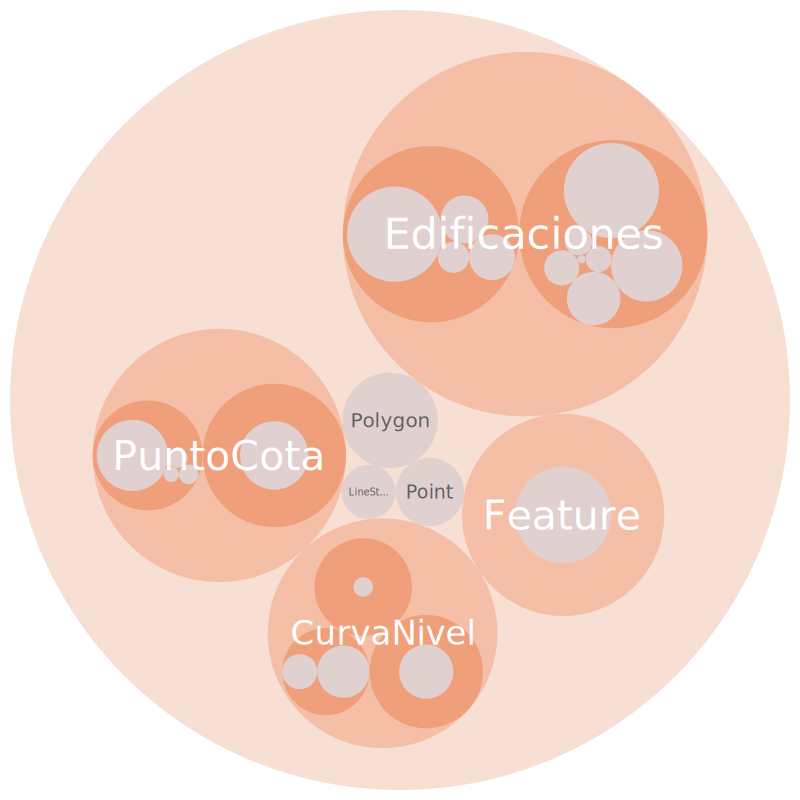
\includegraphics[width=\textwidth]{imagenes/capitulo5/class-hierarchy-TFM}
		\caption{}
	\end{subfigure}       
	\begin{subfigure}[h]{0.33\textwidth} 
		\includegraphics[width=\textwidth]{imagenes/capitulo5/class-hierarchy-TFM-2}
		\caption{}
	\end{subfigure}
\begin{subfigure}[h]{0.33\textwidth} 
	\includegraphics[width=\textwidth]{imagenes/capitulo5/class-hierarchy-TFM-3}
	\caption{}
\end{subfigure}
\begin{subfigure}[h]{0.33\textwidth} 
	\includegraphics[width=\textwidth]{imagenes/capitulo5/class-hierarchy-TFM-4}
	\caption{}
\end{subfigure}
	\caption{Visualizar la ontología completa en GraphDB}
	\label{fig:class}
\end{figure}


Seguidamente, comenzamos la realización de las consultas de SPARQL y GeoSPARQL, clasificando las consultas de acuerdo a la geometría que contiene. Al principio comenzaremos con consultas más sencillas, hasta la obtención de la consulta que nos permita saber las \textbf{edificaciones que se encuentran a una cierta altura o cercanas a una cota} con el fin de obtener un fin, para ello, hemos considerado dos geometrías que nos pueden dar la misma aproximación de altura pero con geometrías distintas, una con puntos y otra con líneas.



%Lo primero, disponemos de la información geográfica espacial referente a Ogíjares con respecto edificaciones, curvas de nivel y cotas de altura. Con esta información, que fue seleccionada para un fin, queremos saber las edificaciones que se encuentran a una cierta altura con el fin de obtener un objetivo, para ello, hemos cogido dos geometrías que nos pueden dar la misma aproximacion pero con geometrías distintas, una con puntos y otra con líneas.

\subsection{Consultas donde intervienen solo polígonos}

\textit{Ejemplo 1}. Consulta que obtiene los tres primeros polígonos de Edificaciones que pertenecen a la clase TipoEdificaciones y son EDI (Edificación). Con esta consulta queremos obtener las edificaciones que están edificadas. 

\vspace*{0.2cm}

\begin{lstlisting}
SELECT ?x ?p
WHERE {
	?x rdf:type geo:EDI .
	?polygon geo:asWKT ?p
}
\end{lstlisting}

\vspace*{0.2cm}

En la figura \ref{fig:salida3} podemos observar los GID correspondientes y sus coordenadas asociadas.

\begin{figure}[H]
	\centering
	\includegraphics[width=1\linewidth]{imagenes/capitulo5/salida3}
	\caption{Salida de la consulta para el Ejemplo 1}
	\label{fig:salida3}
\end{figure}

\textit{Ejemplo 2}. Consulta que obtiene la geometría específica de WKT mediante el operador \texttt{geof:sfEquals}. Con esta consulta queremos obtener las Edificaciones correspondientes a una determinada ubicación.

\vspace*{0.2cm}

\begin{lstlisting}
SELECT ?f
WHERE {
	?f geo:asWKT ?fWKT .
	
	FILTER (geof:sfEquals(?fWKT, '''
	POLYGON ((446050.16 4107127.71, 446053.42 4107107.66, 446029.09 4107103.93, 446028.94 4107104.69, 446027.13 4107112.67, 446041.35 4107115.08, 446039.91 4107125.24, 446050.16 4107127.71)) 
	'''^^geo:wktLiteral))
} 
\end{lstlisting}

\vspace*{0.2cm}

En la figura \ref{fig:salida3} podemos observar cómo una ubicación exacta solo referencia a una geometría. Además, si pinchamos sobre ella nos devuelve información relevante al respecto (figura \ref{fig:info-salida}).

\begin{figure}[H]
	\centering
	\includegraphics[width=1\linewidth]{imagenes/capitulo5/salida2}
	\caption{Salida de la consulta para el Ejemplo 2}
	\label{fig:salida2}
\end{figure}

\begin{figure}[H]
	\centering
	\includegraphics[width=1\linewidth]{imagenes/capitulo5/info-salida}
	\caption{Información de la consulta para el Ejemplo 2}
	\label{fig:info-salida}
\end{figure}

Para comprobar que corresponde dicha salida con la información de la ontología, veamos el fragmento correspondiente al GID 181064.

\vspace*{0.2cm}

\begin{lstlisting}
<!-- http://www.opengis.net/ont/geosparql#181064 -->

<geo:asWKT rdf:datatype="http://www.opengis.net/ont/geosparql#wktLiteral"> POLYGON ((446050.16 4107127.71, 446053.42 4107107.66, 446029.09 4107103.93, 446028.94 4107104.69, 446027.13 4107112.67, 446041.35 4107115.08, 446039.91 4107125.24, 446050.16 4107127.71))
</geo:asWKT>
\end{lstlisting} 

\subsection{Consultas donde intervienen solo puntos}

\textit{Ejemplo 3}. Consulta que obtiene los cinco primeros puntos de PuntoCota con una cota de 700 metros de altitud, y que pertenecen a la clase ContextoPuntoCota y son DEP(Depresión). Con esta consulta queremos obtener los Puntos de Cota que tiene más de una cierta altura y son depresiones.

\vspace*{0.2cm}

\begin{lstlisting}
SELECT DISTINCT ?point ?pointCota
WHERE {
	?point rdf:type geo:DEP ;
	geo:tieneCota ?pointCota ;
	
	FILTER (?pointCota > 700)
}
\end{lstlisting}

\vspace*{0.2cm}

En la figura \ref{fig:salida5} podemos observar los cinco primeros puntos obtenidos y sus correspondientes cotas.

\begin{figure}[H]
	\centering
	\includegraphics[width=1\linewidth]{imagenes/capitulo5/salida5}
	\caption{Salida de la consulta para el Ejemplo 3}
	\label{fig:salida5}
\end{figure}

\textit{Ejemplo 4}. Consulta que obtiene la geometría específica de WKT mediante el operador \texttt{geof:sfWithin}. Con esta consulta queremos obtener los Puntos de Cota que están dentro de una determinada ubicación, pudiendo obtener un único valor o varios. 

\vspace*{0.2cm}

\begin{lstlisting}
SELECT ?f
WHERE {
	?f geo:asWKT ?fWKT .
	
	FILTER (geof:sfWithin(?fWKT, '''
	MULTIPOINT ((446228.92 4108432.53))
	'''^^geo:wktLiteral))
} 
\end{lstlisting}

En la figura \ref{fig:salida7} podemos observar que solo se encuentra dentro de esa ubicación una cota.

\begin{figure}[H]
	\centering
	\includegraphics[width=1\linewidth]{imagenes/capitulo5/salida7}
	\caption{Salida de la consulta para el Ejemplo 4}
	\label{fig:salida7}
\end{figure}

\subsection{Consultas donde intervienen solo líneas}

\textit{Ejemplo 5}. Consulta que obtiene  la geometría específica de WKT mediante el operador \texttt{geof:sfEquals}. Con esta consulta obtener las Curvas de Nivel correspondientes a una ubicación exacta.

\vspace*{0.2cm}

\begin{lstlisting}
SELECT ?f
WHERE {
	?f geo:asWKT ?fWKT .
	
	FILTER (geof:sfEquals(?fWKT, '''
	LINESTRING (440972.52 4106237.28, 440972.4 4106232.04, 440972.15 4106226.75, 440967.68 4106204.44, 440964.32 4106205.94, 440963.48 4106208.23, 440962.08 4106213.03, 440960.59 4106219.28, 440959.9 4106224.26, 440958.99 4106229.78, 440958.44 4106234.81, 440958.11 4106240.01, 440958.05 4106245.3, 440958.04 4106250.86, 440958.16 4106255.93, 440958.41 4106261.44, 440959.21 4106266.96, 440960.76 4106272.24, 440971.61 4106288.61, 440974.39 4106281.06, 440974.85 4106275.81, 440974.77 4106270.3, 440972.52 4106237.28)
	'''^^geo:wktLiteral))
} 
\end{lstlisting}

En la figura \ref{fig:salida1} podemos observar cómo una ubicación exacta solo referencia a una geometría.

\begin{figure}[H]
	\centering
	\includegraphics[width=1\linewidth]{imagenes/capitulo5/salida1}
	\caption{Salida de la consulta para el Ejemplo 5}
	\label{fig:salida1}
\end{figure}

Para comprobar que corresponde dicha salida con la información de la ontología, veamos el fragmento correspondiente al GID 172684.

\vspace*{0.2cm}

\begin{lstlisting}
<!-- http://www.opengis.net/ont/geosparql#172684 -->

<geo:asWKT rdf:datatype="http://www.opengis.net/ont/geosparql#wktLiteral">LINESTRING (440972.52 4106237.28, 440972.4 4106232.04, 440972.15 4106226.75, 440967.68 4106204.44, 440964.32 4106205.94, 440963.48 4106208.23, 440962.08 4106213.03, 440960.59 4106219.28, 440959.9 4106224.26, 440958.99 4106229.78, 440958.44 4106234.81, 440958.11 4106240.01, 440958.05 4106245.3, 440958.04 4106250.86, 440958.16 4106255.93, 440958.41 4106261.44, 440959.21 4106266.96, 440960.76 4106272.24, 440971.61 4106288.61, 440974.39 4106281.06, 440974.85 4106275.81, 440974.77 4106270.3, 440972.52 4106237.28)
</geo:asWKT>
\end{lstlisting}

\subsection{Consultas donde intervienen líneas y puntos}

\textit{Ejemplo 6}. Consulta que obtiene las cincos primeras geometrías (líneas y puntos) que tienen una cota superior a 700 metros de altitud. Con esta consulta estamos quedándonos con las alturas correspondientes a un valor.

\vspace*{0.2cm}

\begin{lstlisting}
SELECT ?f
WHERE {
	?f geo:tieneCota ?fCota
	FILTER (?fCota > 700)
}
\end{lstlisting}

En la figura \ref{fig:salida4} podemos observar los GID obtenidos.

\begin{figure}[H]
	\centering
	\includegraphics[width=1\linewidth]{imagenes/capitulo5/salida4}
	\caption{Salida de la consulta para el Ejemplo 6}
	\label{fig:salida4}
\end{figure}

\textit{Ejemplo 7}. Consulta que obtiene las cincos primeras geometrías (líneas y puntos) que tienen una cota superior a 720 metros de altitud y muestra tanto su ubicación con WKT como su cota. Con esta consulta estamos quedándonos con las alturas correspondientes a un valor, y mostrando el valor de su cota y su ubicación. En la figura \ref{fig:salida6} se observa el resultado.


\vspace*{0.2cm}

\begin{lstlisting}
SELECT DISTINCT ?point ?pointWKT ?pointCOTA
WHERE {
	?point 	geo:asWKT ?pointWKT ;
	geo:tieneCota ?pointCOTA .
	FILTER (xsd:double(?pointCOTA) > 720)
}
\end{lstlisting}


\begin{figure}[H]
	\centering
	\includegraphics[width=1\linewidth]{imagenes/capitulo5/salida6}
	\caption{Salida de la consulta para el Ejemplo 7}
	\label{fig:salida6}
\end{figure}



Hay que tener en cuenta que hay muchas maneras de hacer las consultas, por lo que para realizar una consulta, no es necesario realizarla de la misma forma que estamos haciéndola nosotros.




%\underline{GEOF:sfEquals}


\subsection{Consultas donde intervienen polígonos y puntos}

\textit{Ejemplo 8}. Consulta que obtiene las cincos primeras geometrías de puntos cercanas a un metro del GID de Edificaciones 889549. Con esta consulta nos estamos quedando los Puntos de Cota que están cercanos al GID 889549, con esto es posible obtener la altura asociada a dicha edificación.

\vspace*{0.2cm}

\begin{lstlisting}
SELECT ?f
WHERE {
	geo:889549 geo:asWKT ?WKT .
	?f rdf:type sf:Point ;
	geo:asWKT ?fWKT .
	
	FILTER (?fGeom != ?WKT)
}
ORDER BY ASC(geof:distance(?cWKT, ?fWKT, uom:metre))
\end{lstlisting}

En la figura \ref{fig:salida9} podemos apreciar los 5 puntos más cercanos al 889549.

\begin{figure}[H]
	\centering
	\includegraphics[width=1\linewidth]{imagenes/capitulo5/salida9}
	\caption{Salida de la consulta para el Ejemplo 8}
	\label{fig:salida9}
\end{figure}

%\underline{GEOF:WITHIN}

\textit{Ejemplo 9}. Consulta que obtiene las cincos primeras geometrías de polígonos cercanas a un metro de las geometrías de puntos. Con esta consulta nos estamos quedando con las Edificaciones que están a más de 700 metros de altitud.

\vspace*{0.2cm}

\begin{lstlisting}
SELECT ?p
WHERE {
	?p rdf:type sf:Polygon ;
	geo:asWKT ?pWKT .
	?f rdf:type sf:Point ;
	geo:tieneCota ?pointCota ;
	geo:asWKT ?fWKT .
	
	FILTER (?pointCota > 700)
}
ORDER BY ASC(geof:distance(?pWKT, ?fWKT, uom:metre))
\end{lstlisting}

En la figura \ref{fig:salida9} podemos apreciar los 5 edificios más cercanos a una cota superior a 700 metros de altura.

\begin{figure}[H]
	\centering
	\includegraphics[width=1\linewidth]{imagenes/capitulo5/salida11}
	\caption{Salida de la consulta para el Ejemplo 9}
	\label{fig:salida11}
\end{figure}

\subsection{Consultas donde intervienen polígonos y líneas}

\textit{Ejemplo 10}. Consulta que obtiene las cincos primeras geometrías de líneas cercanas a un metro del GID de Edificaciones 889549. Con esta consulta nos estamos quedando las Curvas de Nivel que están cercanos al GID 889549, con esto es posible obtener la altura asociada a dicha edificación.

\vspace*{0.2cm}

\begin{lstlisting}
SELECT ?f
WHERE {
	geo:889549 geo:asWKT ?WKT .
	?f rdf:type sf:LineString ;
	geo:asWKT ?fWKT .
	
	FILTER (?fGeom != ?WKT)
}
ORDER BY ASC(geof:distance(?cWKT, ?fWKT, uom:metre))
\end{lstlisting}

En la figura \ref{fig:salida9} podemos apreciar las 5 líneas más cercanos al edificio 889549.

\begin{figure}[H]
	\centering
	\includegraphics[width=1\linewidth]{imagenes/capitulo5/salida10}
	\caption{Salida de la consulta para el Ejemplo 10}
	\label{fig:salida10}
\end{figure}

\subsection{Consultas donde intervienen polígonos, líneas y puntos}

%geof:distance

\textit{Ejemplo 11}. Consulta que obtiene las cincos primeras geometrías más cercanas a un metro del GID de Edificaciones 889549. Con esta consulta nos estamos quedando con las características más cercanas al GID 889549.

%Find the 3 closest features to feature my:C, where computations are based on my:hasExactGeometry.
%Encuentre las 3 características más cercanas para presentar my: C, donde los cálculos se basan en my: hasExactGeometry.

\vspace*{0.2cm}

\begin{lstlisting}
SELECT ?f
WHERE {
	geo:889549 geo:asWKT ?WKT .
	?f geo:asWKT ?fWKT .
	
	FILTER (?fGeom != ?WKT)
}
ORDER BY ASC(geof:distance(?cWKT, ?fWKT, uom:metre))

\end{lstlisting}

\begin{figure}[H]
	\centering
	\includegraphics[width=1\linewidth]{imagenes/capitulo5/salida8}
	\caption{Salida de la consulta para el Ejemplo 11}
	\label{fig:salida8}
\end{figure}




Acabamos de comprobar como es posible obtener de manera eficaz los GID ubicados en el mapa, sin embargo \textit{¿dónde se encuentran exactamente ubicados?} A continuación, contestamos esta pregunta.\\


\textit{\textbf{Nota}: Las consultas se encuentran en el directorio \texttt{consultas}.}



%geo:sfContains



\section{Visualización de la Información Geográfica}
\label{ch:visualizacion}


\begin{figure}[H]
	\centering
	\includegraphics[width=1\linewidth]{imagenes/capitulo5/R1}
	\caption{Página principal del mapa Web}
	\label{fig:r1}
\end{figure}

Con los GID que antes hemos mostrado, no conocemos información acerca de a que GID está haciendo referencia \textit{¿entonces como podemos visualizarlo y ubicarlos en un mapa?} La respuesta es muy simple con \texttt{Leaflet} que es una biblioteca JavaScript de código abierto ampliamente utilizada para crear aplicaciones de mapeo Web. Para hacer uso de ella se suele usar principalemente Java, sin embargo, nosotros hemos hecho uso de R al haber encontrado un tutorial que explica muy bien su utilización con Shiny\footnote{Shiny es un framework Web para R.} (\url{https://rstudio.github.io/leaflet/shiny.html}). Para ejecutarla hace falta abrir el fichero en R Studio y pulsar el boton ``Run App''.\\


En las figuras \ref{fig:r1},  \ref{fig:r2}, \ref{fig:r3} y \ref{fig:r4} podemos ver una visualización del mapeo Web realizado para encontrar los GID de nuestros datos en el mapa. En la figura \ref{fig:r1} se observa la página inicial de la aplicación. Con esto, se extiende el uso que se le puede dar a la prueba de concepto, ya que esta aplicación ha permitido que podamos obtener y ubicar en un mapa información.\\



% Para ello nos hemos creado un ejemplo con R.

%En Java hay consultas para trabajar con información espacial, (WorldWindJava)

%Hablar sobre la librería MapView y leafet de Java

%Está hecho con Shiny Web App.



En las figuras \ref{fig:r2}, \ref{fig:r3} y \ref{fig:r4} se observan las geometrías ubicadas en el mapa para las distintas geometrías que tenemos, para ello se ha hecho un ejemplo con cada una de ellas. Por esa misma razón, a partir de la realización de la consulta para obtener los edificios que están a una determinada altura es posible saber de manera gráfica donde se encuentra su ubicación exacta mediante el uso de esta aplicación. No obstante, hemos puesto que se ubique en el mapa las tres geometrías que hemos venido comentando. A continuación, se muestran tres ejemplos, en donde se debe pulsar el botón ``Buscar" para que los ubique en el mapa.

\begin{figure}[H]
	\centering
	\includegraphics[width=1\linewidth]{imagenes/capitulo5/R2}
	\caption{Obtención de la información del GID para Edificaciones}
	\label{fig:r2}
\end{figure}

\begin{figure}[H]
	\centering
	\includegraphics[width=1\linewidth]{imagenes/capitulo5/R3}
	\caption{Obtención de la información del GID para Curvas de Nivel}
	\label{fig:r3}
\end{figure}

\begin{figure}[H]
	\centering
	\includegraphics[width=1\linewidth]{imagenes/capitulo5/R4}
	\caption{Obtención de la información del GID para Puntos de Cota}
	\label{fig:r4}
\end{figure}



\textit{\textbf{Nota}: El código se encuentra en el directorio \texttt{visualizacion}.}\\

%\section{Evaluación de la prueba de concepto}




\section{Conclusiones}

En este capítulo, se ha presentado la prueba de concepto realizada para la Web Semántica Geoespacial en donde se han obtenido los datos del Instituto de Estadística y Cartografía de Andalucía, en concreto la información geoespacial de edificaciones, curvas de nivel y puntos de cota de Ogíjares (Granada) en formato Shapefile. A partir de esa información se ha creado la ontología GEOARES en RDF/OWL y poblado mediante la herramienta Protegé, haciendo uso de unas determinadas reglas. Seguidamente, debido a diversos problemas, se ha hecho uso de la alternativa GraphDB para aplicar las búsquedas mediante los lenguajes de consulta GeoSPARQL y SPARQL. Finalmente, se ha creado una pequeña aplicación de mapa Web para obtener las salidas de las consultas en un mapa y así observar su visualización. Esta prueba de concepto nos ha permitido comprobar cómo la Web Semántica permite hacer uso de diversas herramientas esenciales que facilitan la búsqueda de la información, en este caso de Información Geográfica.







%Gracias a este tipo de archivo podemos generar MDT secundarios: mapas de orientación, de pendiente, cuencas visuales o sencillos archivos de sombreado (\textit{hillshade}), materia prima con la que analizar el territorio. Es por ello que, una vez descargados nuestros datos, ya podemos llevar a cabo el análisis del mapa de sombras para el MDT. Primero lo realizaremos en R, seguidamente en QGIS y, por último, veremos la interacción entre ambas, dejando documentado el proceso, para así poder hacer la evaluación y comparación entre ambas herramientas.







% Uso de la similitud semántica para la recuperación de información geoespacial: https://dialnet.unirioja.es/servlet/tesis?codigo=61960
% http://rua.ua.es/dspace/handle/10045/45811
% https://rua.ua.es/dspace/bitstream/10045/45811/1/tesis_machado_garcia.pdf

% http://www.ciw.cl/material/tw07arodriguez.pdf

% Semántica Geoespacial en la web: https://slideplayer.es/slide/10277009/

% https://nextweb.gnoss.com/busqueda/tag/geoespacial

% Para que es para acceder a datos espaciales en la web
% http://linkedgeodata.org/OnlineAccess
% http://linkedgeodata.org/sparql

% https://www.w3.org/community/geosemweb/wiki/Main_Page
% https://en.wikipedia.org/wiki/Semantic_Geospatial_Web
% https://www.opengeospatial.org/projects/initiatives/gswie
% http://www.personal.psu.edu/faculty/f/u/fuf1/Fonseca-Sheth.pdf

% https://www.researchgate.net/publication/283801501_Geospatial_Semantic_Web
% https://www.researchgate.net/publication/300494545_Geospatial_Data_Interoperability_Geography_Markup_Language_GML_Scalable_Vector_Graphics_SVG_and_Geospatial_Web_Services
% https://www.semanticscholar.org/paper/Supporting-Frameworks-for-the-Geospatial-Semantic-Abdelmoty-Smart/e3998c31905b0d9eebaceddad5040e940caa594a
% https://www.sciencedirect.com/science/article/pii/S1570826809000468

% https://www.mdpi.com/journal/ijgi/special_issues/geospatial_semantics

% Documentos Scholar sobre "geospatial semantic web": https://scholar.google.es/scholar?q=geospatial+semantic+web&hl=es&as_sdt=0&as_vis=1&oi=scholart

% http://www.irisa.fr/LIS/ferre/sparklis/?title=Core%20English%20DBpedia&endpoint=http%3A//servolis.irisa.fr/dbpedia/sparql&sparklis-query=%5BVId%5DReturn%28Det%28An%281%2CModif%28Select%2CUnordered%29%2CClass%28%22http%3A//dbpedia.org/ontology/Database%22%29%29%2CNone%29%29&sparklis-path=D
% http://www.irisa.fr/LIS/ferre/sparklis/?endpoint=http%3A//servolis.irisa.fr/dbpedia/sparql&sparklis-query=%5BVId%5DReturn%28Det%28An%287%2CModif%28Select%2CUnordered%29%2CClass%28%22http%3A//dbpedia.org/ontology/Place%22%29%29%2CNone%29%29&sparklis-path=D

% https://www.sciencedirect.com/science/article/pii/S1570826809000468

% http://www.geonames.org/ontology/documentation.html

% https://ieeexplore.ieee.org/document/1656068

% https://www.chnt.at/the-geospatial-semantic-web-as-foundation-for-knowledge-networks-of-cultural-heritage/

% http://geoknow.eu/Welcome.html


%Un SIG ha sido ampliamente utilizado por una variedad de aplicaciones, muchas bases de datos geográficas han sido desarrolladas por diferentes programas y software. Sin embargo, sigue siendo un gran problema compartir estos datos geoespaciales y usarlos para el desarrollo de aplicaciones SIG. No es que los datos no estén disponibles, hay una gran cantidad de datos geográficos almacenados en diferentes lugares y en diferentes formatos, pero la reutilización de datos para nuevas aplicaciones y el intercambio de datos son tareas abrumadoras debido a la heterogeneidad de los sistemas existentes en términos de conceptos de modelado de datos, técnicas de codificación de datos y estructuras de almacenamiento, etc.\\

%Hay dos problemas que resultan directamente de la no interoperabilidad de las bases de datos. Uno es el cambio en la exactitud de los datos. Después de que los datos se conviertan de un formato a otro, pueden ocurrir problemas como la precisión de coordenadas, errores de omisión, nombres de atributos faltantes o incorrectos y una topología incorrecta. El segundo problema es la inversión de tiempo y dinero para la conversión de datos. Se ha desperdiciado mucho dinero y tiempo en la conversión de datos o en el desarrollo de herramientas de conversión de datos.\\

%La interoperabilidad de datos significa la capacidad de utilizar una variedad de formatos de datos. Los datos geoespaciales interoperables pueden ser utilizados por diferentes tipos de programas y aplicaciones. Con datos geoespaciales interoperables, los usuarios deben poder solicitar, acceder e integrar datos fácilmente sin importar dónde se almacenen los datos (local o remotamente). La interoperabilidad de los datos geoespaciales es extremadamente importante para las aplicaciones geoespaciales, ya que existían grandes cantidades de datos espaciales de diferentes formatos geográficos y hay una mayor demanda de reutilización de estos datos espaciales existentes para la toma de decisiones. La interoperabilidad de los datos geoespaciales elimina las barreras para el intercambio de datos y permite a los usuarios acceder, mapear, visualizar y analizar directamente datos con diferentes formatos de datos espaciales. Los datos geoespaciales interoperables hacen posible la distribución rápida de información y el intercambio entre departamentos.\\


%\section{Web Semántica Geoespacial}

% http://www.mclibre.org/consultar/xml/lecciones/web-semantica.html#spatial-data

%\subsection{Arquitectura Web Semántica Geoespacial}

% se debería de hacer una mención a la web semántica tradicional o la web tradicional


% 

%https://mangomap.com/gis-mapping

% ---------------------------------------------------------------------------

%¿qué datos cogemos?
%
%Descargamos datos de aquí: https://www.juntadeandalucia.es/institutodeestadisticaycartografia/bcadescargas/
%- Base Cartográfica de Andalucía (2) > Base Cartográfica de Andalucía (shape) > Ogíjares
%
%Para saber más información acerca de los datos: https://www.juntadeandalucia.es/institutodeestadisticaycartografia/prodCartografia/bc/modelo.htm
%
%Para instalar Google Maps en QGIS
%https://mappinggis.com/2018/03/como-anadir-mapas-base-en-qgis-3-0-openstreetmap-google-carto-stamen/
%
%
%- Elemento Edificaciones (poligonal): Se agrupan en esta capa varios elementos que conforman edificaciones. Se debe tener en cuenta que el nucleo urbano engloba en áreas grandes a las edificaciones.
%
%- Elemnto ParqueJardinP (puntual): Recinto en el interior de una población destinado a prados, jardines y arbolado
%para recreo y ornato. 

%-----

%Se trabajará con información  geoespacial, concretamente con archivos en formato Shapefile. 
%
%La mejora de las herramientas se enfocará únicamente a las destinadas a la generación (QGIS que permitirá llevar la información  de los shapefile hacia hojas de cálculo y Protegé permitirá llevar la información  de los shapefile hacia documentos en formato RDF), y consumo GraphBD que permite la visualización de archivos en formato RDF y visualización (aplicación en R que permite la visualización de archivos en formato RDF),  y como lenguaje de consulta geoespacial, este estándar es GEOSPARQL.
%
%Finalmente, todos los datos generados mediante las herramientas mejoradas, se publicarán en un repositorio disponible, el cual dará lugar al: repositorio de Datos Enlazados Ecuatoriano el cual debe permitir su acceso al público en general. 


% ----

%Para hacer uso de este lenguaje de consulta, es necesario utilizar herramientas que permitan GeoSPARQL, no sólo SPARQL. Es por eso que la herramienta Protegé carece de funcionamiento para este tipo de consultas
%
%Como hemos comentado anteriormente, la herramienta Protegé nos permite construir contologías de manera más sencilla y rápida, sin embargo, también nos ofrece herramienta para realizar consultas con SPARQL. No obstante, carece de funcionamiento para las consultas de GeoSPARQL. En el siguiente apartado, hablaremos también 
%
%en este caso, 

%---

%\section{Resumen del capítulo}





